\chapter{RESULTS} \label{chapter:results}
The results basically provide answers to the following research questions, raised in section \ref{sec:researchQuestions} :
    \begin{enumerate}
        \item To what extent the system is able to capture the harmonic lead sheet constraints.
        \item The impact of the different soloing styles on the proposed system.
        \item The suitability of the system to apply the proposed approach in real time settings.
    \end{enumerate}

For this purpose, two test jazz standards were examined (``All of me" and ``Au Privave") in different settings, simulating two extreme cases: 
    \begin{itemize}
        \item No notes: In this case, the human solo channel consists of consecutive rest occurrences. 
        \item Random notes: Here, randomly chosen notes within a range of two octaves, comprise the solo channel.
    \end{itemize} of no notes (case 1) and random notes (case 2) in the human solo channel. In this chapter, the system's responses in those scenarios are analyzed and examined, acquiring knowledge and feedback about the approach proposed. Sound samples of the system's output are publicly available on Github\footnote{\url{https://github.com/theatina/iJazzARTIST}}.
    
    \section{Jazz Standards} \label{sec:jazzStandards}
    Jazz standards are musical compositions that play an important role in jazz musicians' musical repertoire. A ``jazz standard” is held in continuing esteem and is commonly used as the basis of jazz arrangements and improvisations. 
    
    Not all jazz standards were written by jazz composers. Many are originally Tin Pan Alley popular songs, Broadway show tunes or songs from Hollywood musicals – the Great American Songbook. In Europe, jazz standards and "fake books" may even include some traditional folk songs (such as in Scandinavia) or pieces of ethnic music (such as gypsy melodies) that have been played with a jazz feel by well known jazz players. A commonly played song can only be considered a jazz standard if it is widely played among jazz musicians. The jazz standard repertoire has some overlap with blues and pop standards.
    
    The two jazz standards chosen to test the approach presented are the following : 
    \begin{itemize}
        \item All of Me ( popular song and jazz standard written by Gerald Marks and Seymour Simons in 1931 )
        \item Au Privave ( bebop jazz standard composed by Charlie Parker in 1951 )
    \end{itemize}    
    
    For the procedure, all the measures of each jazz standard were repeated four times in a row (forming the four quarters that are analyzed below), resulting in 40 measures in total. This construction allows us to perform thorough examination of the system's response by comparing and analyzing the respective generated chords.


    
    \section{Compliance with Lead Sheet Chords}
    A lead sheet is a musical composition comprising a chord progression and a melody line. A chord is a group of notes played simultaneously producing a distinct sound as a group. Because of their compactness, lead sheets provide a common means of representing music for both professionals and amateurs, often in the form of large collections known as ``fake books” \cite{keller2010impro}. The lead sheet does not explicitly describe the chord voicings, voice leading, bass line or other aspects of the accompaniment. Instead, these are specified later by an arranger or improvised by the performers \cite{benward1997music}. A lead sheet is often used by jazz musicians; one or more performers will play the melody line, while the rest of the ensemble improvises an accompaniment based on the chord progression given in the chord symbols, followed by an improvised solo also based on the chord progression.

    In this section, the ability of the system to capture the harmonic guidelines of the lead sheet is studied, which is the answer to the first question, stated in \hyperref[sec:researchQuestions]{Research Questions} above. The examination is conducted at pitch class set (PC-set) (set of all pitches with the same note name or its enharmonic equivalent) level, 
    that is, the chart chords and the system's interpretations, are indicated by their pitch class representation.  
    
    To examine the impact of the training on the system's harmonic compliance, data from different epochs (59 and 1251) were collected and presented below. 
    
    %------TABLES------%
    \input{chapters/tables/5_1.txt}
    \input{chapters/tables/5_2.txt}
    \input{chapters/tables/5_3.txt}
    \input{chapters/tables/5_4.txt}
    %------TABLES------%
        
    
    In tables \ref{tab:aom_chords_e59} and \ref{tab:aom_chords_e1251}, the chord symbols and the system's responses in the case of the ``All of me" jazz standard are shown, when no solo and random solo was provided. Similarly, tables \ref{tab:ap_chords_e59} and \ref{tab:ap_chords_e1251} present the respective results for the ``Au privave" jazz standard.

    The information on the system's performance and outcomes that can be drawn from the tables, lead to some conclusions. For example, regarding ``All of me", as presented in Tables \ref{tab:aom_chords_e59} and \ref{tab:aom_chords_e1251}, in most of the time-steps, the system was able to reflect the exact harmonic description in the lead sheet chart. The harmonic deviations which were mostly observed in the first few measures, are attributed to the system's delay in building memory for its decisions.
   

    \begin{figure}[!htb] 
    \centering
    \begin{tabular}{c}
        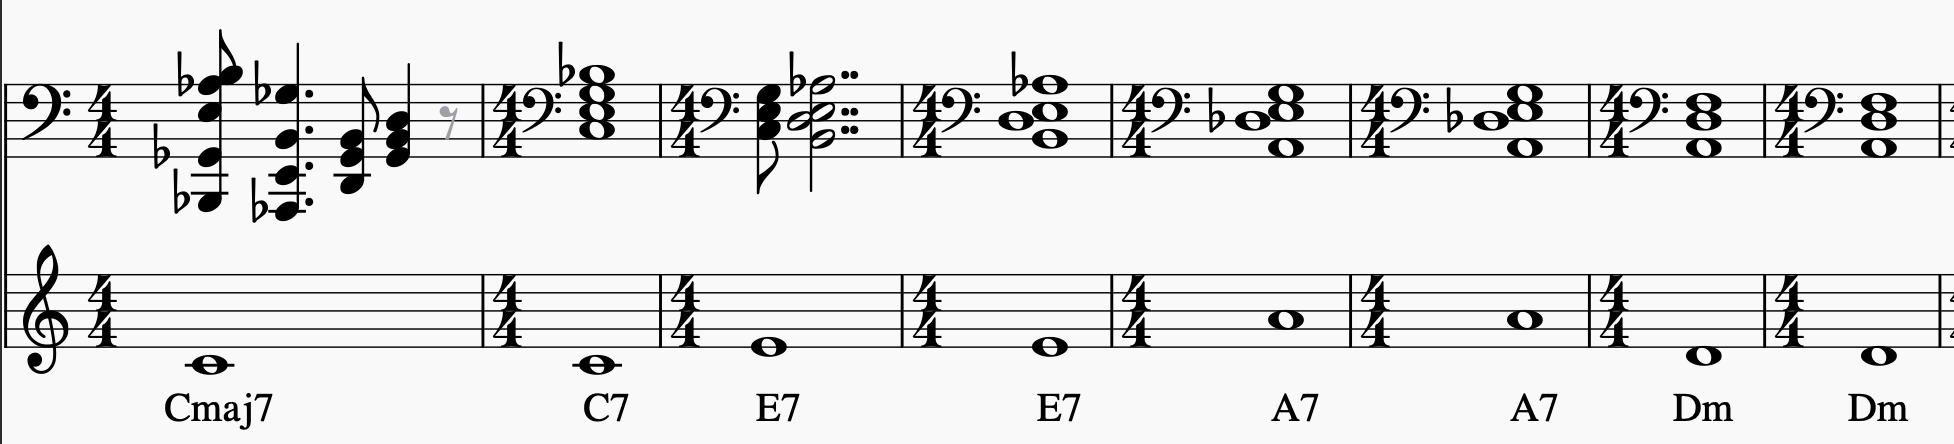
\includegraphics[width=0.9\textwidth]{media/aom_rand_bars1-8.png} \\
        (a) Bars 1-8 \\
        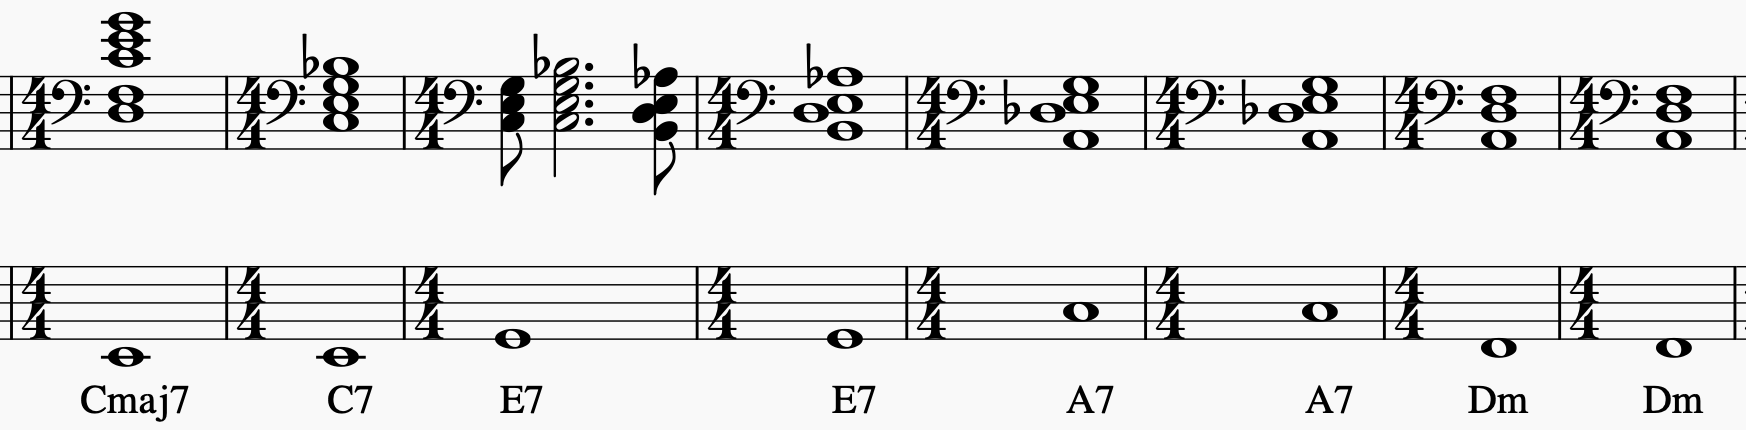
\includegraphics[width=0.85\textwidth]{media/aom_rand_bars33-40.png} \\
        (b) Bars 33-40
    \end{tabular}
    \caption{First 8 measures (a) and last 8 measures (b) of system-generated chords over the respective lead sheet chords for ``All of Me'' with random solo part.}
    \label{fig:aom_beginning_comparison}
    \end{figure}

    Figure \ref{fig:aom_beginning_comparison}, shows the first 8 (1-8) and final 8 (33-40) measures of the system's output chords, under the ``All of me" jazz standard lead sheet in real time. In this instance, the solo was a sequence of random notes, omitted from the system's output depiction in the figure. The first three chords of the first measure, indicate the aforementioned delay of the system to capture and comply with the given constraints, as they comprise inaccurate choices for the respective lead sheet chord. Additionally, in some cases, the system has shown inability to follow the unexpected chord changes, such as the transition from the Cmaj7 (C major seventh) chord ( [0,4,7,11] ) to the E7 (E seventh) chord ( [2,4,8,11] ), shown in measures 2-3 ( \ref{fig:aom_beginning_comparison}(a) ) and 34-35 ( \ref{fig:aom_beginning_comparison}(b) ) of the figure. 

    %Finally, compared to epoch 59 ( Table \ref{tab:aom_chords_e59} ), after the 1251st epoch of training, the lead sheet chords are   \ref{tab:aom_chords_e1251} shows better ...

    Similarly, the output chords of the system over the ``Au privave" jazz standard lead sheet chords are shown in Tables \ref{tab:ap_chords_e59} and \ref{tab:ap_chords_e1251}, following a resemblant compliance pattern but demonstrating fewer inaccurate interpretations.

    \section{Variability}
    
    The system's generated chords of each piece in each scenario, are expected to differ, as the human solo improvisations are considered to have an impact on the system's response, which is examined through direct comparison between the two pieces in each case.

    \input{chapters/tables/5_5.txt}
    \input{chapters/tables/5_6.txt}
    \input{chapters/tables/5_7.txt}
    \input{chapters/tables/5_8.txt}

    In order to study the variability of the system-generated chords, quartile similarities were computed and shown in Tables \ref{tab:aom_quartile_59} and \ref{tab:aom_quartile_1251} regarding the ``All of me" piece and Tables \ref{tab:ap_quartile_59} and \ref{tab:ap_quartile_1251} for the ``Au Privave" jazz standard. More explicitly, this similarity indicates the normalized percentage of different chords per time step during the accompaniment process, over four repetitions(``quartiles") of each chart, with random and without solo.  
    
    It was calculated that in ``All of Me”, the percentage of system-generated chords that are different between random and no solo for epoch 59 is only 2\%, which rises to 60\% after training the system for 1251 epochs, showing that the impact of the solo in the system's response is more remarkable in early epochs, compared to the effect of its presence as epochs progress. In ``Au Privave” the same percentage ranges from 74\% after epoch 59 and reaches 84\% at epoch 1251, leading to the conclusion that the presence of the solo has greater impact on the system's generations for this particular piece. The results of the comparison between each improvisation scenario which are depicted in the tables mentioned above, led to the conclusions extensively discussed below.

    In ``All of Me” under the setting of no solo, only the first repetition differs from the remaining three, in both epochs 59 and 1251 of the system's training, as shown in Tables \ref{tab:aom_quartile_59} and \ref{tab:aom_quartile_1251}, in their first rows and columns. However, as observed from the similarity in the case of random solo, the response in the early epoch was not affected in general, while in the late epoch the influence of the solo is shown to be strong. Overall, the artificial agent's variability in the presence of random solo, concerning ``All of me", indicates the system's responsiveness to the human agent's input, after being trained for multiple epochs (1251 in this case). In contrast, regarding ``Au Privave", the system has generated variations of the lead sheet chart for each iteration, even from the early epoch ( 59 ), as well as demonstrated more conspicuous variability after more epochs (1251). 

    Another means of comparison in the terms of the system's variability, is the total number of different voicings generated for each chord symbol of the chart, with variations of their layouts being note doublings or inversions to name a few. 

    \begin{figure}
    \centering
    \begin{tabular}{cc}
        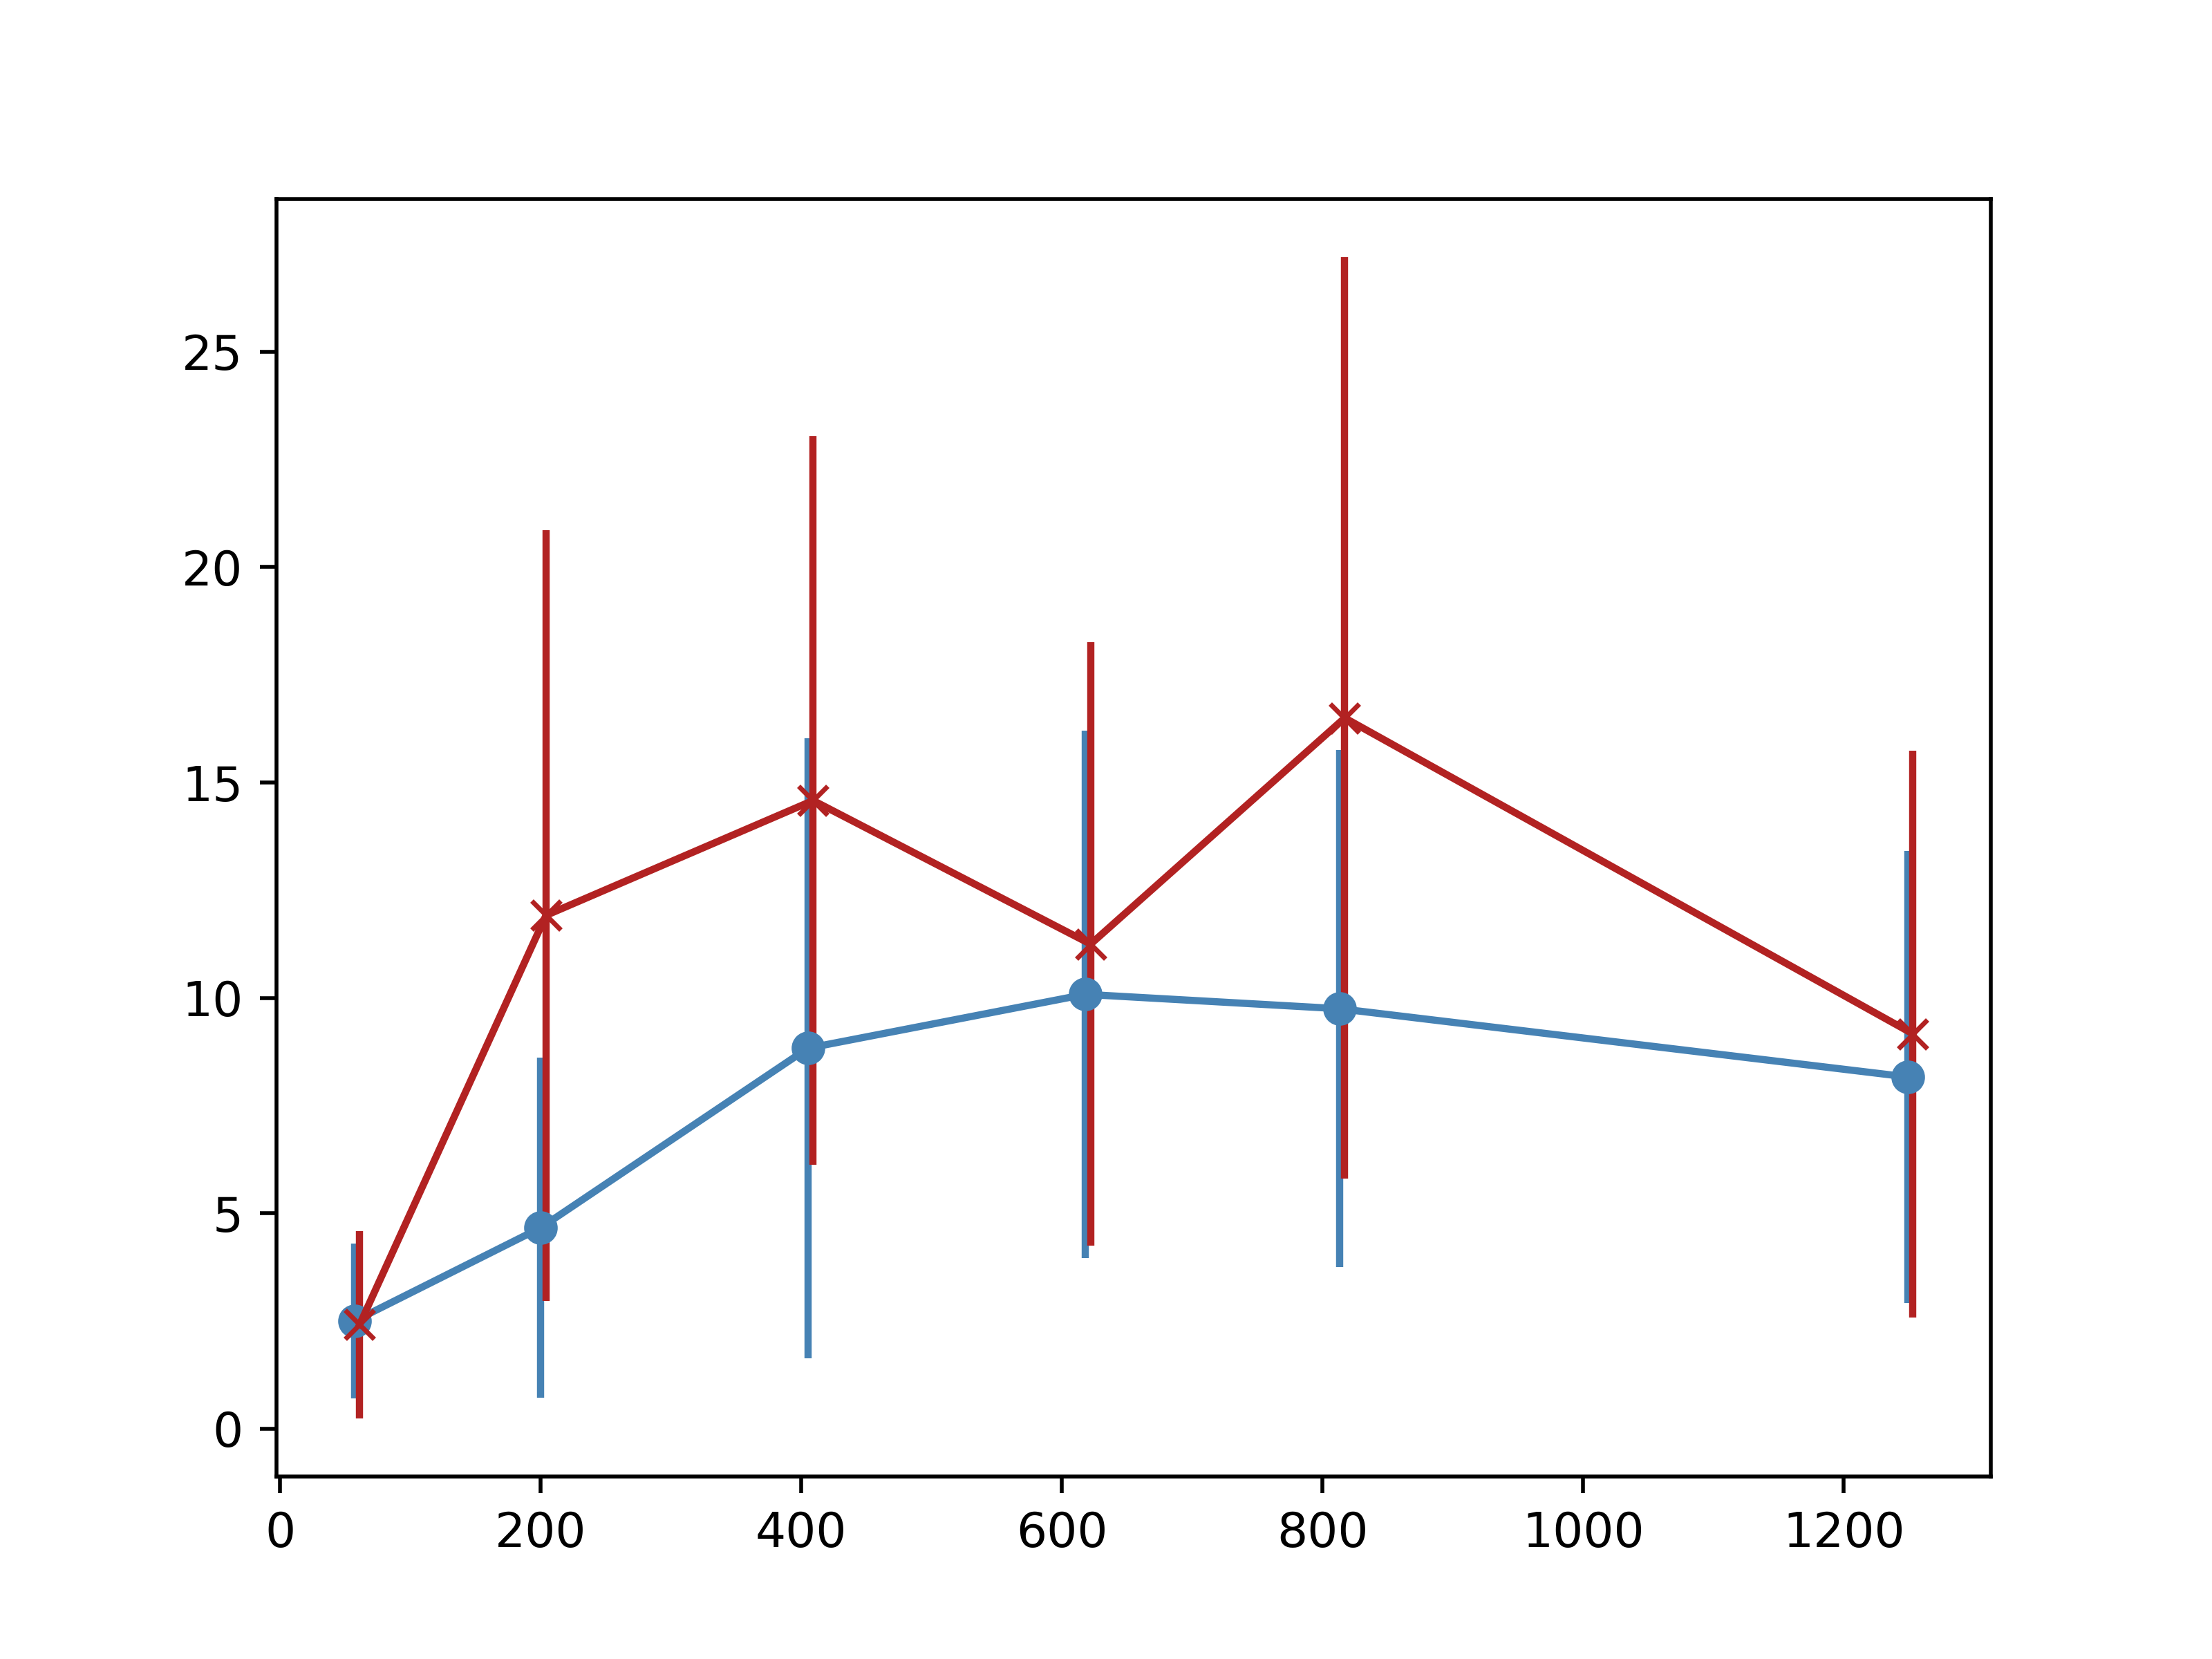
\includegraphics[width=0.5\textwidth]{media/aom_voicings_errorbars.png} & 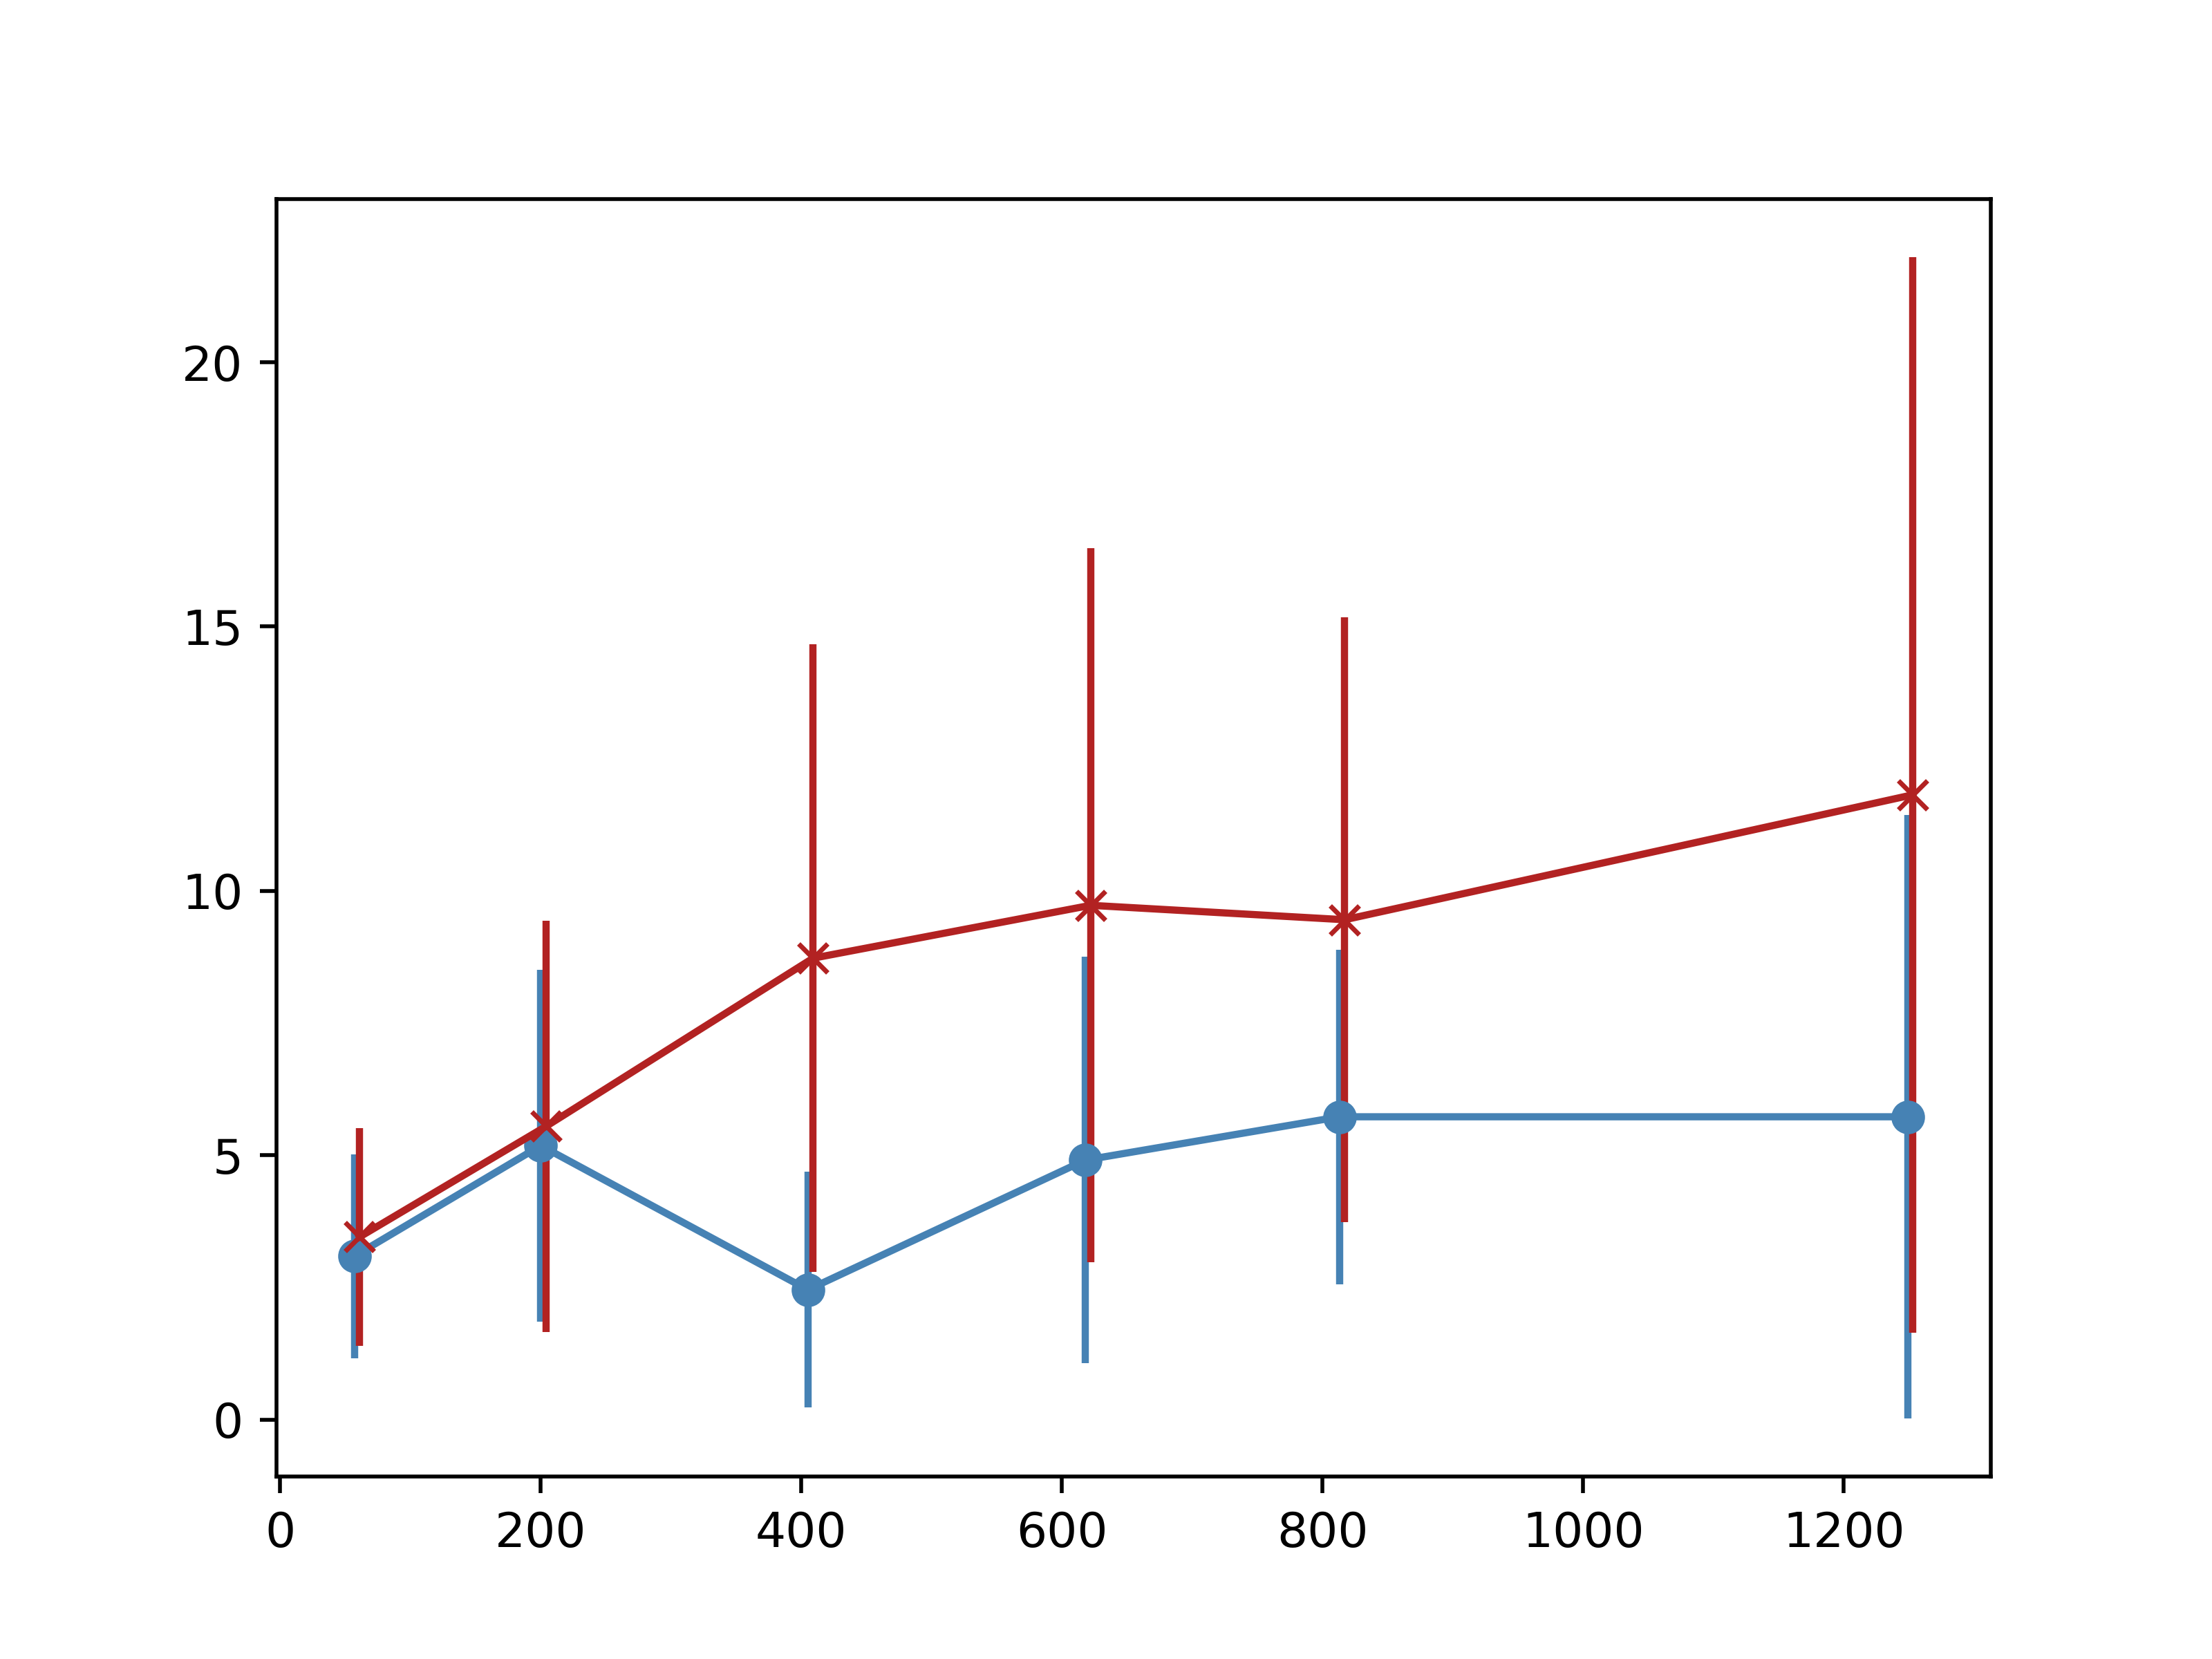
\includegraphics[width=0.5\textwidth]{media/ap_voicings_errorbars.png} \\
        All of me & Au Privave
    \end{tabular}{}
    \caption{Error-bars of different voicings generated for each chord label in the chart over a set of sampled epochs, in the presence of random solo (red) and absence thereof (blue).}
    \label{fig:voicings}
    \end{figure}{}

    In Figure \ref{fig:voicings}, the different voicings for each chord label of the chart are shown, over a set of randomly chosen epochs from the total epochs of the system's training. As indicated in the figure, in ``All of me", at the 59th epoch of the training, the system  generated approximately 2.5 variations of chord voicings and proved to be independent of the solo presence, which is not the case in later epochs, as the variability dependence on the solo increases as the epochs progress. Also, in ``Au Privave", the growing tendency of dependency on the solo is more evident, as the epochs increase. Finally, thorough concurrent examination of Figures \ref{fig:val_loss} and \ref{fig:voicings}, leads to the conclusion that there is a correlation between the objective function loss and the system's adaptability to the human solo, with lower loss values (further training) providing greater variability of the system. 
    
    % \clearpage
    % \section{Audio Samples}
    % \begin{center}

\includemedia[
  transparent,
  passcontext,
  addresource=./chapters/soundFiles/jack5.mp3,
  flashvars={source=./chapters/soundFiles/jack5.mp3},
]{\color{blue}\framebox[0.4\linewidth][c]{Audio sample}}{APlayer.swf}
% \caption{Audio sample from the generated accompaniment for the the `` " jazz standard with no solo.}
\end{center}